\section{Results: the context-reliance family under attack}
\label{sec:results}

\subsection{One design rule explains most of what we found}

Stated first, then supported: \textbf{a defense that works by shifting trust
from the model's parameters toward the retrieved text is correct when the text
is merely stale and dangerous when an attacker owns it.}

This family is large. It includes
ParamMute~\cite{huang-2025-parammute}, CK-PLUG~\cite{bi-2025-parameters},
SpARE~\cite{zhao-2024-steering}, COIECD~\cite{yuan-2024-discerning} and
SHIFT~\cite{li-2026-shift}. All were published as fixes for knowledge
conflict, and all were validated against the incidental threat model only. The
family's shared idea is reasonable for the problem it was built for. When a
retrieved document disagrees with the model's memory, the document is usually
newer, so trust the document. The idea becomes a liability the moment the
document is written by an adversary, because the defense instructs the model to
trust the one thing the adversary controls.

\begin{table}[t]
\caption{Context-reliance defenses against corpus poisoning, each read against
its own undefended arm in the same run. "Clean" is the defense's own published
benefit. "Saturation" is 100\% poisoned context. Bold clears that run's
minimum detectable change.}
\label{tab:family}
\small
\begin{tabular}{@{}lrrrr@{}}
\toprule
\textbf{Defense} & \textbf{$n$} & \textbf{mdr} & \textbf{Clean} &
\textbf{Saturation} \\
\midrule
ParamMute & 1409 & 5.3 & \textbf{+9.3} & \textbf{-4.2} \\
CK-PLUG   &  800 & 7.0 & \textbf{-10.1}$^{\dagger}$ & \textbf{-9.9} \\
SpARE     &  500 & 8.9 & \textbf{+14.2} & \textbf{-10.2} \\
COIECD    &  400 & 9.9 & -0.8 & -1.8 \\
\bottomrule
\end{tabular}
\\[2pt]
{\footnotesize $^{\dagger}$CK-PLUG's control fires on memorisation rate rather
than accuracy, so its clean cell reports that metric.}
\end{table}

SpARE is the cleanest case because its control and its conviction are the same
measurement. Steering toward the context is worth \textbf{+14.2\pp} when the
context is honest and costs \textbf{-10.2\pp} when it is attacked. Both ends
clear the 8.9\pp threshold. The sign flips.

ParamMute shows the same shape on a larger sample. Its benefit on clean context
is +9.3\pp. At saturation it is 4.2\pp \emph{below} the undefended model, and
across the full dose range it loses 13.5\pp more accuracy than doing nothing at
all.

CK-PLUG's behaviour is the most extreme we measured, and it appears on a
different metric. Under BadRAG sentiment steering~\cite{xue-2024-badrag}, which
tries to make the model answer in a negative tone, the undefended model adopts
the attacker's framing 0.0\% of the time at every dose. CK-PLUG adopts it
78.2\% of the time with a single poisoned passage out of ten, and 99.0\% at
full dose. The defense does not fail to stop the attack. It carries it.

\begin{figure*}[t]
\centering
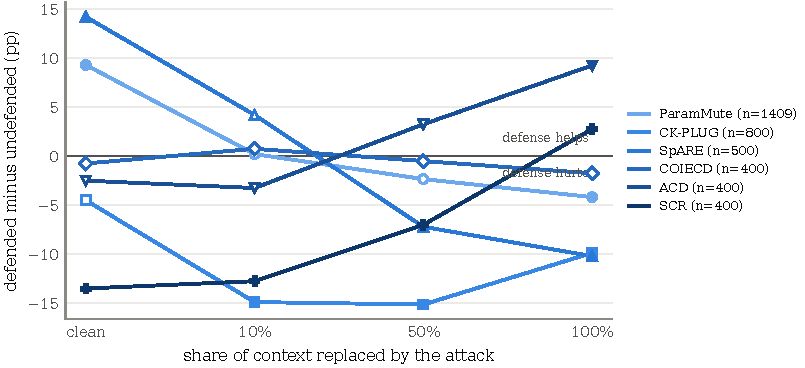
\includegraphics[width=0.82\textwidth]{figures/fig4_dose_response}
\caption{Every retrieval-cell defense against corpus poisoning, measured as the
defended arm minus its own undefended arm in the same run. Zero means the
defense changed nothing. Filled markers are resolvable at $p < .05$ by Fisher's
exact test, hollow are not. Three patterns are visible. SpARE and ParamMute
start above zero and cross it, which is the sign flip. CK-PLUG and SCR sit
below zero almost everywhere, costing accuracy before the attack arrives. ACD
is the only line that rises, and Table~\ref{tab:acd} shows that rise does not
survive a change of payload.}
\label{fig:dose}
\end{figure*}

\subsection{The scope condition}

The rule is not that suppressing parametric memory is always harmful. We can
state when it is.

\textbf{Suppressing the model's prior knowledge hurts only where that prior
knowledge held the right answer.} Against BadRAG's denial-of-service variant,
which makes the model refuse rather than answer wrongly, ParamMute is strongly
protective. With one poisoned passage in ten the undefended model refuses
52.4\% of the time and holds 27.0\% accuracy. ParamMute drops refusal to 0.2\%
and restores accuracy to 57.4\%, within 2.4 points of its own clean baseline.
Across the realistic range of one to five poisoned passages, the undefended
model averages 25.8\% accuracy and ParamMute averages 57.6\%.

The mechanism is the same in both cases. ParamMute suppresses the model's
memory. When memory held the correct answer, that suppression destroys it. When
the attack works by driving the model into refusal, suppressing memory removes
the conflict that triggered the refusal. \textbf{One mechanism, two signs,
selected by whether the memory was right.} We predicted little effect here and
were wrong, which is why the scope condition is in the paper.

\subsection{The payload class decides, not the attack label}

ACD~\cite{kim-2024-adaptive} was the best result in our campaign. It discounts
tokens the context makes uncertain, and against corpus poisoning it is the only
method that both reads a clean document and resists a poisoned one. At
saturation it is \textbf{+9.2\pp} above the undefended arm ($p < 0.0001$) and
on clean context it is \textbf{+53.5\pp} above answering with no document at
all.

We then ran the same defense, same items, same doses, against false evidence.

\begin{table}[t]
\caption{ACD against two payload classes, $n=400$, mdr 9.9\pp. The defense is
unchanged. Only the form of the planted passage differs.}
\label{tab:acd}
\small
\begin{tabular}{@{}lrr@{}}
\toprule
\textbf{Comparison at saturation} & \textbf{Corpus poisoning} &
\textbf{False evidence} \\
\midrule
vs.\ undefended  & \textbf{+9.2} ($p{<}0.0001$) & +3.0 ($p{=}0.059$) \\
vs.\ no retrieval & +0.5 ($p{=}0.91$) & \textbf{-4.0} ($p{=}0.0499$) \\
\bottomrule
\end{tabular}
\end{table}

\textbf{The protection collapses.} Against the incoherent payload, ACD restores
the no-retrieval floor exactly. Against the fluent payload it ends up
resolvably \emph{below} that floor: the defended model does worse than a model
given no document at all.

The reason is visible in the method. ACD keys on the uncertainty a passage
induces. An optimized token string is incoherent and raises uncertainty, so ACD
discounts it. A fluent sentence asserting a plausible wrong answer lowers
uncertainty, so ACD trusts it more.

This has a practical consequence. \textbf{The cheaper and more natural-looking
attack is the stronger one.} For COIECD's undefended arm, false evidence cuts
accuracy roughly twice as far as gradient-optimized corpus poisoning at every
dose, falling to 15.2\% at 10\% dose against 26.5\% for corpus poisoning. The
field's attention to optimized adversarial passages is not matched by their
effectiveness.

\subsection{Two payloads, three defenses, three outcomes}
\label{sec:payloads}

ACD is not the only method whose behaviour depends on the form of the planted
passage. We ran the three context-reliance defenses whose corpus-poisoning
results are already in Table~\ref{tab:family} against false evidence as well,
each against its own undefended arm over the same items at the same doses.
Predictions for all three were committed to version control before any of them
ran.

\begin{table}[t]
\caption{The same three defenses against two payload classes. Excess damage is
the defended arm's clean-to-saturation collapse minus the same collapse in its
own undefended arm; positive means the defense lost more accuracy than doing
nothing would have.}
\label{tab:payloads}
\small
\begin{tabular}{@{}lrrr@{}}
\toprule
\textbf{Defense} & \textbf{$n$} & \textbf{Corpus poisoning} &
\textbf{False evidence} \\
\midrule
ParamMute & 1409 & \textbf{+13.5} & \textbf{+12.3} \\
CK-PLUG   &  800 & \textbf{+5.4}  & +0.4 \\
COIECD    &  400 & +1.0           & -1.2 \\
\bottomrule
\end{tabular}
\end{table}

\textbf{ParamMute is harmful against both, and the way it fails is the
finding.} A defense worth +9.7\pp on honest context costs 12 to 13 points more
than doing nothing once an adversary writes the context, and it does not matter
whether the adversary writes gibberish or prose. What does change is how well
ParamMute does its own job. Its suppression of the wrong parametric answer
falls from \textbf{-42.5\pp} under corpus poisoning to \textbf{-8.8\pp} under
false evidence. The reason is structural. Under corpus poisoning the wrong
answer has one source, the model's memory, so inhibiting memory removes it.
Under false evidence it has two, memory and the planted passage, and ParamMute
touches only one of them. \textbf{The attack duplicated the answer into the
channel the defense does not operate on.}

\textbf{CK-PLUG is harmful against one payload and flat against the other}, and
the shape matters more than the sign. Under corpus poisoning its cost grows
with the attack: -4.5\pp on clean context, then -14.9 and -15.1 once poison is
present. Under false evidence it is a constant offset of about -4.4\pp at every
dose including the clean one, and no cell clears the 7.0\pp threshold. CK-PLUG
pays a fixed price for being switched on; corpus poisoning amplifies that price
and false evidence does not.

\textbf{COIECD is inert against both.} Eight comparisons, largest 1.8\pp
against a 9.9\pp threshold, no $p$ below 0.20. Its memorisation-rate
suppression does shrink roughly threefold under false evidence, which is what
an entropy constraint should do when the planted passage agrees with the prior
rather than contradicting it, but that signal sits below threshold and we
record it as directional rather than as a result.

\subsection{A comparison we decline to make}

The three results invite a ranking across payload classes, and we committed in
advance to treating one as a falsifier: if any defense did \emph{better}
against false evidence than against corpus poisoning, then "these defenses fail
because they trust the context" would not be the mechanism. CK-PLUG does, at
+0.4\pp against +5.4\pp.

We do not think that reading survives inspection, and we say so rather than
quietly dropping the test. The two payloads are not equally strong on the
undefended arm. False evidence is roughly twice as damaging at every dose: for
CK-PLUG's undefended arm, 23.0\% against 39.2\% at 10\% dose, and for COIECD's,
15.2\% against 26.5\%. Excess damage is a difference of two collapses, and when
the undefended arm has already collapsed there is less room left for a defense
to make things worse.

\textbf{Excess-damage comparisons across payload classes are therefore
confounded by attack strength and should not be read as a ranking.} Within a
payload, against the control measured beside it in the same run, every
comparison in this section stands. We state the limit because the alternative
is to report a falsifier as passed when the instrument cannot support it.

One measurement limit belongs here for the same reason. Under false evidence
the planted passage asserts the same string the model would have recalled, so
the parametric-answer rate cannot distinguish a model that remembered from one
that copied. They produce identical output. That is the attack's design rather
than a flaw in the metric, and it means ParamMute's residual 58.8\% cannot be
split between the two paths. An arm that plants the \emph{gold} answer instead
would separate them.

\subsection{Asking the model to judge the document}

SCR~\cite{huang-2024-trust} is the only method we ran whose design anticipates
an adversary. It shows the model its own no-context answer, the document, and
the answer the document supports, and asks the model to judge which to believe.

It does help at saturation, +2.8\pp over the undefended arm ($p = 0.025$), and
it does genuinely read the document, scoring 41.2\pp above no-retrieval on
clean context. \textbf{It pays 13.5 points on clean data to buy that 2.8.} The
cost is resolvable at every dose below saturation and is roughly five times the
benefit. A defense deployed permanently and attacked occasionally is a poor
trade at that exchange rate.

SCR's parametric-answer rate climbs 22.8, 33.8, 35.8, 52.5 across the dose
range, converging on the closed-book rate of 55.8. Both SCR and ACD slide from
the document toward memory as the attack grows. SCR simply destroys more
correct answers on the way.
